\section{Image Polarimetry in Biomedical Field} \label{sec:chp4-sec5}
Image polarimetry refers to different approaches to describe the propagation of polarized light, its interactions with the optical system, and its medium polarized properties.
The Stokes and Mueller systems are well suited for polarimetry applications, since first they can document the full, partial and un-polarized state of light and second they provide an intensity measure and experimental data.

The Stokes and Mueller polarimetries refer to measuring the Stokes vector and the Mueller matrix, respectively.
These systems can be used either to highlight the different layers of the tissue by showing diffuse light coming from deeper layers and showing the medium response with different polarized conditions (Stokes polarimetry) or to highlight some medium characteristics (Mueller polarimetry).

Although the polarization filters are employed in a \acf{pd} in order to remove any specular reflection of light and capture the backscattered light from deeper levels of the skin, the full potential of image polarimetry in biomedicine has not been explored~\cite{ghosh2011tissue}.
%Gosh~et al.\,\cite{ghosh2011tissue} summarizes 
%Presumably this is due to the challenges such as~\cite{ghosh2011tissue}: 
%	\begin{itemize}
%	\item Extensive loss of polarization signal as a effect of tissue multiple scattering 
%	\item Complicated nature of polarization effects in tissue
%	\item Measurements difficulty, specially for small polarization signals
%	\item Challenges in analysis and quantification of measured signals or images 
%	\item Complexities in understanding and analyzing the obtained results 
%	\item Lack of detailed information on polarimetric properties of various tissues and their effects on polarized propagation.
%	\end{itemize}
	
Currently, several researchers are pursuing innovative solutions in the filed of image polarimetry.
A comprehensive summary of current research in polarimetry and it's problems is provided by Ghosh~et al.\,\cite{ghosh2011tissue}.
%Ghosh~et al.\,\cite{ghosh2011tissue} provided a good summary on the current stage of the research in polarimtery and its problems.
Polarimetry systems can be used either for tissue imaging or analyzing the tissue's optical characteristics.
We categorized the applied polarimetry systems into three groups: (i) partial Stokes polarimeters, (ii) Stokes polarimeters, and (iii) Mueller polarimeters.
The techniques in the first two categories are used to define the polarization state of the backscattered light from the object and the last one is used to detect the optical properties of the sample.
The aforementioned groups and their related studies are discussed in the following.


%However the Stokes-Mueller polarimetry is more suited for polarimetry applications due to two reasons. First the polarized light after interaction with the medium could be fully, partial or un-polarized and Jones calculus is only applicable for fully polarized light state.
%Second intensity measurements of polarized lights and experimental data are more desirable and Mueller formalism is based on experimental consideration of intensity measurements.
%Based on mentioned reasons, the Stokes-Mueller polarimetry is explained in the following. 
% Stokes-Mueller polarimetry system contains two major elements; \textit{PSA}, polarization states analyser and \textit{PSG}, polarization states generator. The \textit{PSA} contains a set of elements which analyse the polarization state of incoming light and \textit{PSG} contains the elements which generate the polarization states. Three main subcategory of polarimetry are introduced by \cite{goldstein2003polarized}, which includes:
%\begin{itemize}
%	\item Rotating element polarimetry \\
%	The Stokes vector and Mueller matrix parameters are measured here with rotating the polarized elements (polarizer, retarder). 	
%	\item Oscillating element polarimetry \\
%	Which rotates the polarization of light using some electro or magneto-optical device such as liquid crystal cell. 
%	\item Phase modulation polarimetry \\
%	These polarimeters use devices that vary in retardance in response to an electrical signal.
%\end{itemize} 
%
%However different types of imaging polarimetry systems had implemented in the literature which does not follow the mentioned category exactly. These systems are discussed with their details in section \ref{polState}.
%\input{Chapter4/ImagePolarimetry-LuChip.tex}

%\subsection{Polarimetry Systems in Biomedical field}
%\label{polState}
\subsection{Partial Stokes polarimeters}
Beside the conventional use of cross-polarized filters in dermoscopes, the polarization and polarimetry systems have been used by several researchers as imaging techniques.
This section describes the image polarimeters which were built to create the first two or three Stokes parameters.
	
Jacques et al \cite{Jacques12175282} were among the first researchers to consider analysing polarized images rather than single image for skin imaging.
In their research they proposed the use of two polarized filters.
A polarizer generator was placed in the incident path in order to create the linearly polarized light illumination and polarizer analyser in the detection path.
In this system the angle of the incident was chosen in a way that only backscattered light was collected with the camera.
The authors proposed two image acquisitions: one with the analysing polarizer oriented parallel to the illumination and one with the analyser positioned perpendicular to the illumination.
%The algebraic combination of these images ($I_{pol} = \frac{I_{par}-I_{per}}{I_{par}+I_{per}}$) leads to an image that emphasizes on the superficial skin structures which scattered the light rather than structures that absorb light \cite{Jacques12175282}.
The algebraic combination of these images ($I_{pol} = \frac{I_{\parallel}-I_{\perp}}{I_{\parallel}+I_{\perp}}$) leads to an image (depolarization ratio image) which is sensitive to superficially scattered polarized light and visualizes the disruption of the normal texture of the papillary and upper reticular dermis by skin pathology~\cite{Jacques12175282}. 
The authors used these imaging techniques for the differentiation of clinical images of skin pathologies. 
%The combination of co and cross polarized images $I_{pol}$ in addition to multispectral set up was used by \cite{yaroslavsky2003} as well. This set up was used for detection the boundaries of non melanoma parts with in the lesion. 

Another project based on the first two Stokes parameters was proposed by Anastasiadou~et al.\,\cite{Anastasiadou2008}.
In this work the authors proposed polarimetric imaging for imaging cervical cancers.
Figure.~\ref{fig:SPcervicalcancer} illustrates their proposed systems.
\begin{figure}[h]
\centering
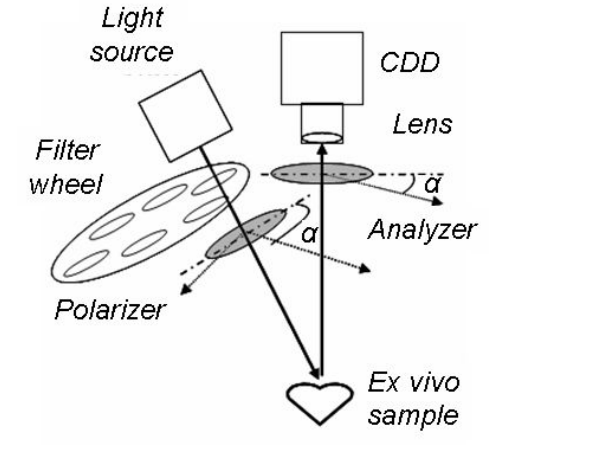
\includegraphics[width = 0.5\textwidth]{Chapter4/Figures/ImagePolarimetryCervicalCancer.png}
\caption[Polarimetry system proposed by \cite{Anastasiadou2008}]{Polarimetric image system proposed by \cite{Anastasiadou2008}.}
\label{fig:SPcervicalcancer}
\end{figure}
\noindent In this figure, $\alpha$ is the azimuth angle and the two images are acquired, $I_{\parallel}$ when the the two polarizers are positioned parallel to each other and $I_{\perp}$ when they are perpendicular.
The proposed system consists of a white light source (150 W halogen bulb), a fiber handle, a filter wheel (three channels 450, 550, and 650 \si{\nano\meter}), a linear polarizer/ analyzer, and finally a CCD camera~\cite{Anastasiadou2008}.
Using this setup, similar to the previous study, the $I_{pol}$ image is calculated as a final image (referred to as $DOP$ in the study).
A classification framework of ex-vivo cervical lesions (76 patients) using the images provided by the proposed imaging system, achieved a \ac{se} of 52-86\% and \ac{sp} of 93\%.
%Examination of the the proposed imaging system on ex-vivo cervical lesions, 76 patients, achieved a \ac{se} of 52-86\% and \ac{sp} of 93\%.
Figure.~\ref{fig:CC-Ex1} illustrates a sample of severe dysplasia comparing images seen under colposcopy and the proposed polarimetry system.
\begin{figure}[h]
\begin{center}
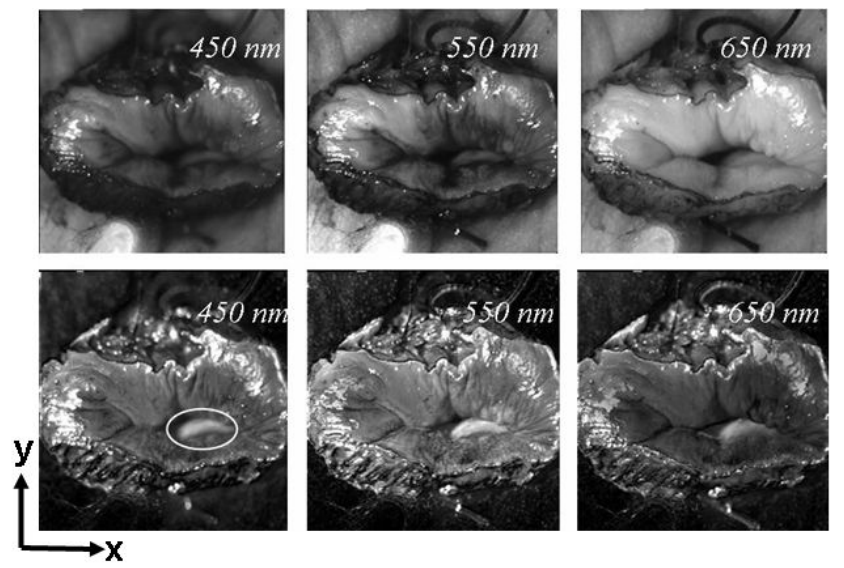
\includegraphics[width = 0.7\textwidth]{Chapter4/Figures/CC-Ex1.png}
\caption[Polarimetry images of ex-vivo cervical dysplasia~\cite{Anastasiadou2008}]{$I_{\parallel}$ and $I_{pol}$, first and second row, respectively. The images were taken with $\alpha = 0$ and at different wavelengths. Images presented by \cite{Anastasiadou2008}.}
\label{fig:CC-Ex1}
\end{center}
\end{figure}
This example was presented as a case, in which the confirmed dysplasia region was not obvious in ordinary images.
However it was clearly noted in the $I_{pol}$ image.

Zhao~et al.\,\cite{zhao2009} introduced another partial polarimetry (spectropolarimetric) imaging system to measure pathological changes of tissue birefringence and structure. 
Figure.~\ref{fig:Zhaosys} shows the proposed system by \cite{zhao2009}.
		\begin{figure}
		\centering
		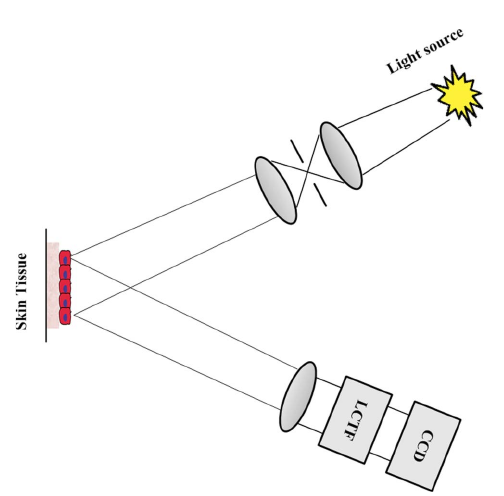
\includegraphics[width = 0.5\textwidth]{Chapter4/Figures/spectropolarimeter.png}	
	\caption[Polarimetry system proposed by \cite{zhao2009}]{The polarimetry system developed by \cite{zhao2009}.}
		\label{fig:Zhaosys}
		\end{figure}	
\noindent This system is composed of an incoherent white light source (halogen) illuminated in a collimated beam at an angle of \ang{25} to the normal of the skin surface and a CCD camera along with a \ac{lctf} used to acquire spectropolarimetric images.
The \ac{lctf} is a bandpass filter that can control the wavelength of the transmitting light and ranges from 400-720\si{\nano\meter}.
The spectropolarimetric images are acquired by manually rotating the \ac{lctf} at \ang{0}, \ang{45}, \ang{90}, and \ang{135} angles.
Using the acquired images the three first Stokes parameters as well as the \ac{dolp} were measured (see Eq.\,\ref{Eq:DP} and Eq.\,\ref{Eq:cStokesmeas}). 
Figure.~\ref{fig:Zhao-ex1} shows an example of the Stokes parameters and \ac{dolp} obtained for chilblain skin at 590 \si{\nano\meter}.
\begin{figure}[t]
\begin{center}
\subfloat[$S_{0}$]{
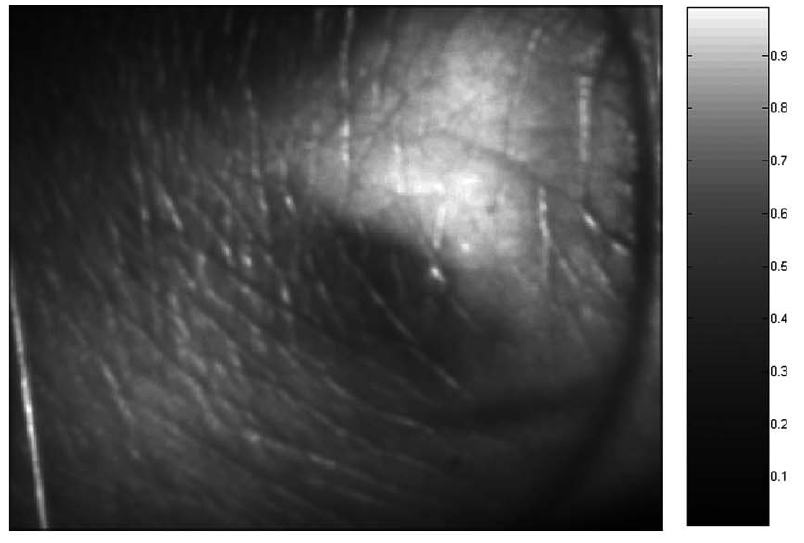
\includegraphics[width = 0.44\textwidth]{Chapter4/Figures/Zhao-ex1-a.png}}\
\subfloat[$S_{1}$]{
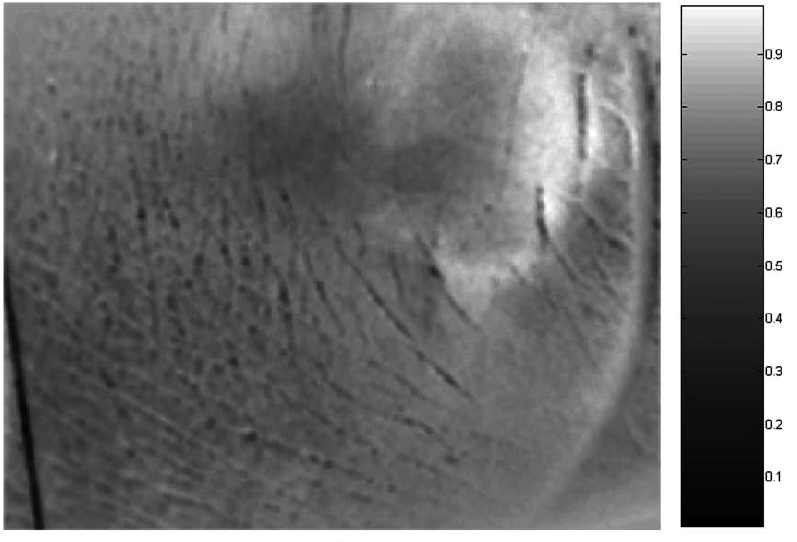
\includegraphics[width = 0.44\textwidth]{Chapter4/Figures/Zhao-ex1-b.png}}\\
\subfloat[$S_{2}$]{
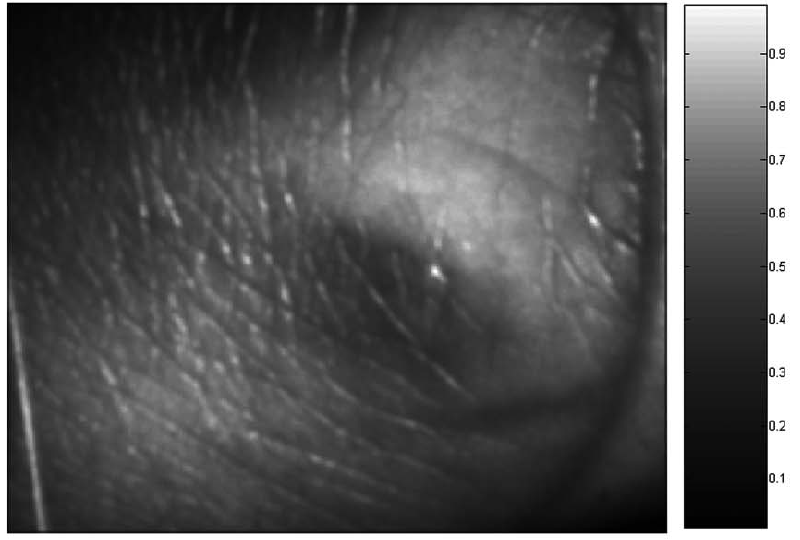
\includegraphics[width = 0.44\textwidth]{Chapter4/Figures/Zhao-ex1-c.png}}\
\subfloat[\ac{dolp}]{
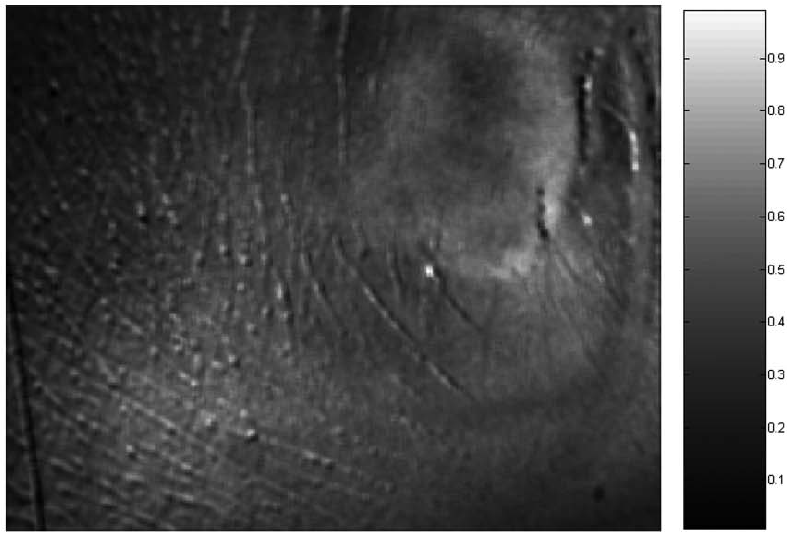
\includegraphics[width = 0.44\textwidth]{Chapter4/Figures/Zhao-ex1-d.png}}
\caption[Polarimetry images of Chilblain skin sample~\cite{zhao2009}]{Chilblain skin sample described by the first three Stokes parameters and \ac{dolp}. Images presented by \cite{zhao2009}.}
\label{fig:Zhao-ex1}
\end{center}
\end{figure} 

Recently, Tchvialeva~et al.\,\cite{tchvialeva2013polarization} proposed using polarization speckle patterns to differentiate and identify skin cancer lesions.
In this research the author proposed calculating the depolarization ratio ($I_{pol}$) from the backscattered speckle patterns using the proposed system shown in Fig.~\ref{fig:TchialevaSys}.
This system is composed of dual cameras, two diode lasers: a blue laser ($\lambda = 407$~\si{\nano\meter}) and a red laser ($\lambda = 663$~\si{\nano\meter}), a diaphragm and a beam splitter.
The speckle patterns are recorded simultaneously by both cameras, one captures the light parallel to the initial polarization and the other captures the light perpendicular to the initial polarization~\cite{tchvialeva2013polarization}.
Figure.~\ref{fig:tchvialeva-ex1} shows examples of polarization speckle patterns for a malignant melanoma, a squamous cell carcinoma, a basal cell carcinoma, a nevus, and a seborrheic keratosis using the blue laser. 
\begin{figure}[tb]
\begin{center}
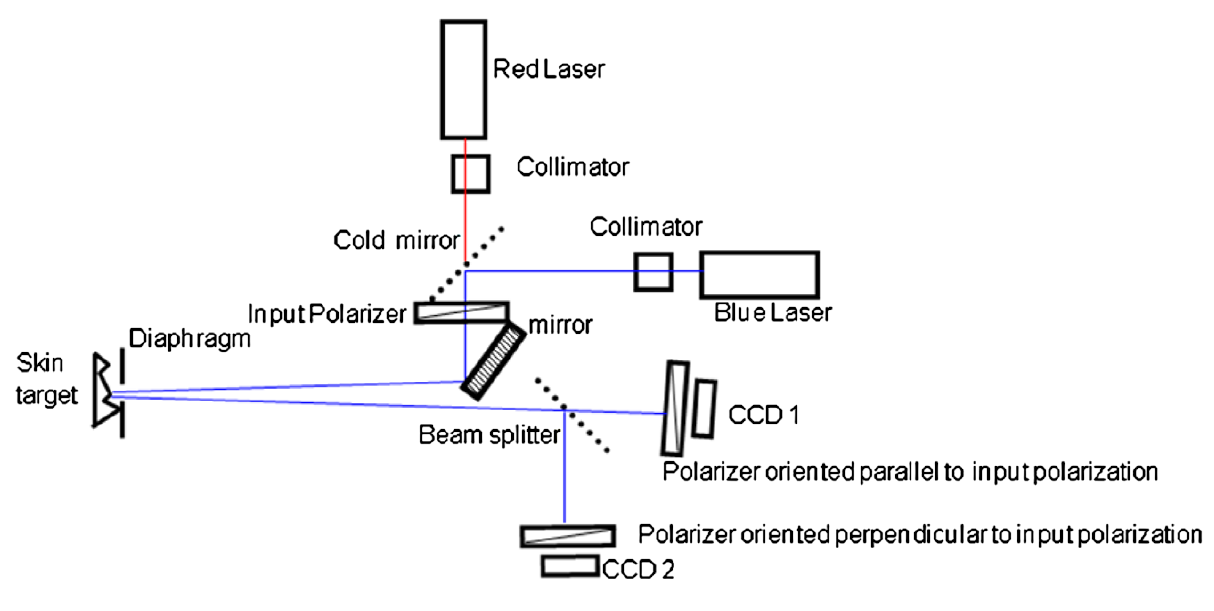
\includegraphics[width= 0.85\textwidth]{Chapter4/Figures/TchvialevaSys.png}
\caption[Polarimetry system proposed by \cite{tchvialeva2013polarization}]{The laser speckle device proposed by \cite{tchvialeva2013polarization}.}
\label{fig:TchialevaSys}
\end{center}
\end{figure}
\begin{figure}
\begin{center}
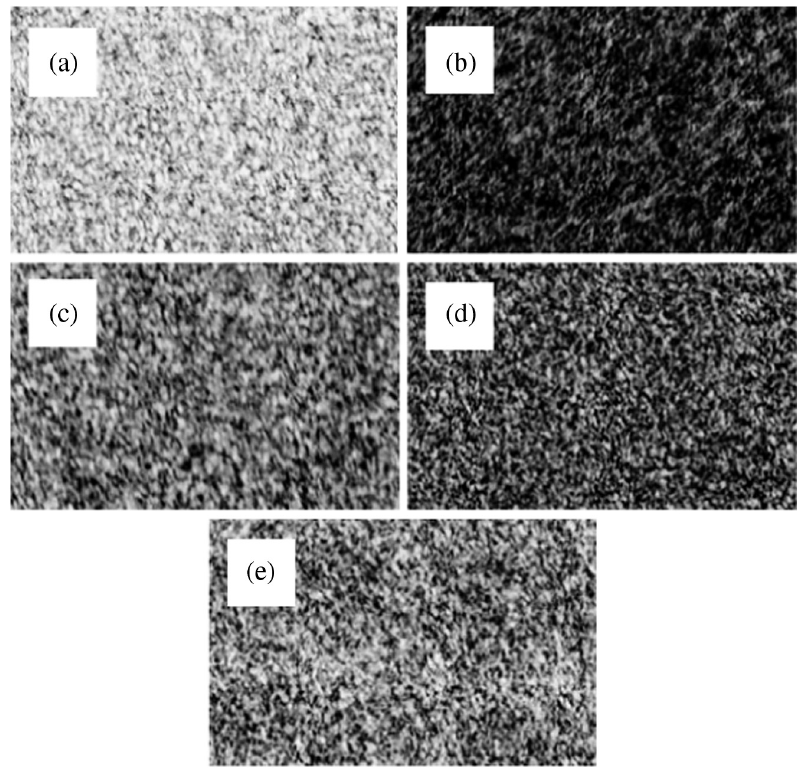
\includegraphics[width = 0.7\textwidth]{Chapter4/Figures/Tchvialeva-ex1.png}
\caption[Speckle polarimetry images of skin lesions]{Examples of polarization speckle patterns of skin lesions using a blue laser (407~\si{\nano\meter}); (a) A malignant melanoma, (b) A squamous cell carcinoma, (c) A basal cell carcinoma, (d) A nevus, and (e) seborrheic keratosis. Images are taken from \cite{tchvialeva2013polarization}.}
\label{fig:tchvialeva-ex1}
\end{center}
\end{figure}
\noindent The authors evaluated their proposed systems on in-vivo 214 skin lesions containing cancer and benign lesions where they reported that statistical moments of the polarization speckle pattern is able to separate malignant melanoma from sebrroheic keratosis, basal cell carcinoma, and squamous cell carcinoma.

	

\subsection{Stokes polarimeters}
A classical approach for measuring the four Stokes parameters was mentioned in Sect.~\ref{sec:chp4-sec3} (see Eq.~\ref{Eq:cStokesmeas}). 
As discussed in the previous section, this approach was partially used in several studies to measure the two or three first Stokes parameters~\cite{tchvialeva2013polarization,zhao2009,Jacques12175282,Anastasiadou2008}.
The choice of partial measurements using the aforementioned setup is because measuring the fourth parameter ($S_{3}$) is relatively more difficult and less accurate than the first three parameters.
This is due to reasons such as: (i) the optical energy absorbed by the retarder should be accounted for when measuring $S_{3}$, (ii) the retarder should be removed and replaced during the acquisition, and  (iii) the perfect alignment of the transmission axis of the polarizer at \ang{45} from the fast axis of the retarder is required.
These factors have made it difficult to accurately measure the $S_{3}$ parameter, using this setup.
To address this problem, Collett\,\cite{collett1984measurement} proposed to use one optical element instead of two.
Collett proposed using a circular polarizer constrcuted by a linear polarizer whose transmission axis is rotated at \ang{45} with respect to the horizontal axis followed by a quarter-wave retarder which its fast axis is parallel to the horizontal direction. 
Using this setup, the three intensities ($I_{C}(\theta)$) are measured when the circular polarizer is rotated at \ang{0}, \ang{45}, and \ang{90} with respect to the horizontal axis and the fourth intensity ($I_{L}(\theta)$) is measured by flipping the linear polarizer to the other side (i.e. the linear polarizer follows the quarter retarder) and keeping its axis parallel to the horizontal axis (i.e. $\theta = \ang{0}$)~\cite{collett1984measurement,ghosh2011tissue}.
The Stokes parameters are calculated from the four measured intensities using the following equation:
\begin{equation}\label{eq:CollettStokes}
\begin{bmatrix}
S_{0} \\ S_{1} \\ S_{2} \\ S_{3} 
\end{bmatrix} = 
\begin{bmatrix}
I_{C}(\ang{0}) + I_{C}(\ang{90}) \\
S_{0} - 2I_{C}(\ang{45}) \\
I_{C}(\ang{0}) - I_{C}(\ang{90})\\
-S_{0} +2I_{L}(\ang{0})
\end{bmatrix}~.
\end{equation}
\noindent This method was used in several researches to measure the Stokes parameters of the light or backscattered light from the tissue~\cite{sankaran1999polarization, ghosh2004depolarization}.

Although this method is more accurate than the classical approach, in order to improve the sensitivity of the measurement it was proposed to use polarization modulation with synchronized detection.
Although such systems provide signals rather than images, they have been used in several studies to measure sample polarization properties~\cite{sankaran2002comparative,wood2008towards}. 
The system proposed by Wood~et al.\,\cite{wood2008towards}, using polarization modulation and a synchronous lock-in-amplifier is shown in Fig.~\ref{fig:pmodulationStokes}.
	\begin{figure}
	\centering 
	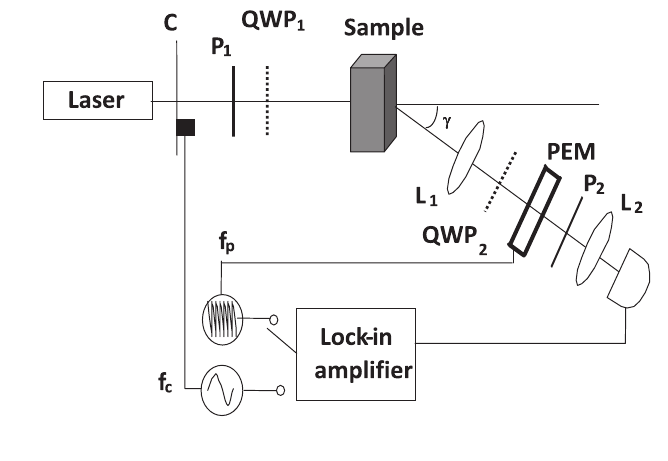
\includegraphics[width = 0.6\textwidth]{Chapter4/Figures/PMSDpolarimetry.png}	
	\caption[Polarimetry system proposed by Wood~et al.\,\cite{wood2008towards}]{Stoke polariemtry system using polarization modulation and a lock-in-amplifier. The image is taken form \cite{wood2008towards}.}
	\label{fig:pmodulationStokes}
	\end{figure}
In such a system, usually un-polarized light passes through the mechanical chopper and then the lock-in amplifier in order to establish its overall signal intensity levels. A linear polarizer ($P_{1}$), with or without a quarter wave plate ($QWP_{1}$) is used as input optics.
This set up is required in order to generate any of the four polarization states.
The detection path consists of a removable quarter wave plate ($QWP_{2}$) with its fast axis oriented at $-45^{\circ}$, a \ac{pem} and a linear polarizer, oriented at $45^{\circ}$.
The linear polarizer converts the \ac{pem} polarization modulation to intensity modulation suited for photodetection.
An interested reader is guided to the original article~\cite{wood2008towards} and Ghosh~et al.\,\cite{ghosh2011tissue} for further details regarding these systems.
%The PEM is a linearly birefringence resonant device, operating in $kHz$ range. The fast axis of the PEM is set to $0^{\circ}$ and its retardation is modulated according to the sinusoidal function $\delta_{PEM} = \delta_{0} \sin(\omega t)$. The $\delta_{0}$ is the user specified amplitude of the maximum retardation of $EPM$.


Besides the above methods for creating a full Stokes polarimetry system, a full Stokes image polarimetry system was proposed by Boulbry~et al.\,\cite{boulbry2006novel}.
The proposed spectro-polarimetric system is based on hemispherical backscattering for analysis of superficial skin lesions.
In order to remove the effect of rough skin backscattering and reflection, the proposed method is constructed with out-of-plane illumination~\cite{ramella2005out}.
The proposed system is composed of sixteen polarized light sources positioned over a hemisphere.
Each light source generates a collimated incident beam of blue, green or red illumination at the center of the hemisphere~\cite{boulbry2006novel}.
Figure \ref{fig:SVhemisphere} shows the position of the illumination source tubes (illuminators) over the hemisphere and the elements within each tube (a tri-color light emission diode, a thin film polarizer and a lens). 
	\begin{figure}
	\subfloat[]{%[width=0.3\textwidth]
	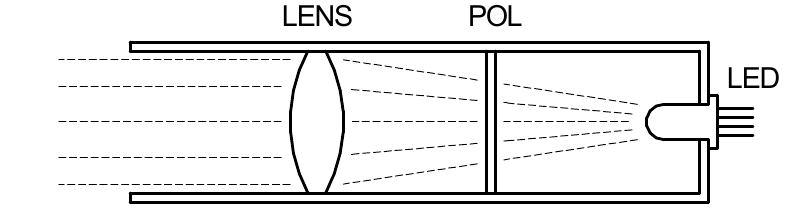
\includegraphics[width = 0.6\textwidth]{Chapter4/Figures/fig1hemisphere.png}
	}\ \hfil
	\subfloat[]{%[width=0.3\textwidth]
    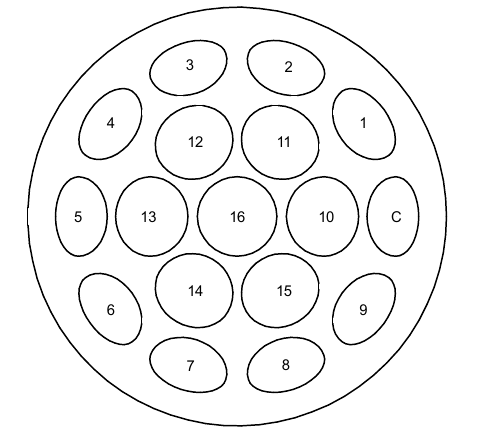
\includegraphics[height = 0.2\textheight , width = 0.35\textwidth]{Chapter4/Figures/fig2hemispher.png}
	}
	\caption[Polarimetric device proposed by \cite{boulbry2006novel}]{(a) The illumination tubeand (b) Sixteen illumination tubes and the camera $C$, on the surface of the hemisphere with respect to the normal of the sample. Images are taken from \cite{boulbry2006novel}.} 			 			    
	\label{fig:SVhemisphere}
	\end{figure}

\noindent A Stokes vector imaging is positioned on the shell at an oblique angle to the sample normal and consists of a 12 bits camera, two \ac{lc} and a fixed polarizer. 
Using seven retardance combinations of rotated crystal retarders, the four Stokes vectors were obtained~\cite{boulbry2006novel} via a least square solution, from which the polarized and unpolarized intensity of the light source as well as the parallel and perpendicular part of the polarized intensity were measured.
The method was only tested on a actinic keratosis and, unfortunately, was not tested on further skin lesions.


%Illuminators 1–9 and the camera are centered 49° from the surface normal, illuminators 10–15 are centered 24° from surface normal, and illuminator 16 is centered on the surface normal. The polarizers in illuminators 5, 10, 13, and 16 aligned 45° from the plane containing them, while those in the rest of the illuminators are aligned in the plane containing the respective illuminator and the surface normal.

%The authors used their implemented system for measuring the Stokes parameters and respectively the un-polaized image. They also suggest to divide the polarized part of the measurements into two categories of reference polarized intensity and cross-polarized reference intensity.  
%	
%	The measurement of four Stokes parameter was discussed in Sec. \ref{StokesMeasurement}. The explained set up was originally proposed by Collett et al. \cite{collett1984measurement}. This method was used by other researchers, such as \cite{ghosh2003depolarization,sankaran1999polarization,zhao2009,boulbry2006novel}, however when accurate quantification of the intrinsic tissue characteristics is required, a more sensitive approach should be considered. The sensitivity of the measurements can be improved by using a polarization modulation in combination with synchronous detection \cite{coa2004balanced,vitkin2002effects,studinski2000methodology,guo2006angular}. 
%	
%  	In \cite{coa2004balanced}, they demonstrate that it is possible to reduce the intensity noise and also direct measurements of Stokes parameters by using a amplitude or polarization modulation in combination with a phase-locked detector. 
%  	
% \cite{vitkin2002effects} used polarization modulation with a synchronize detection in the perpendicular and backscattering orientations to detect the scattered light from the liquid turbid samples containing varying amounts of left and right isometric forms of a chiral sugar. Their research was aimed towards non-invasive techniques of glucose sensing in diabetic patients.   
%
%A schematic of the experimental polarimetry system employing polarization modulation and synchronous detector with reference to \cite{guo2006angular,ghosh2011tissue} is shown in Fig.\ref{fig:PMSDpolarimetry}. In such a system, usually un-polarized light is passes through the mechanical chopper and then the lock-in amplifier in order to establish the overall signal intensity levels. A linear polarizer ($P_{1}$), with or without a quarter wave plate ($QWP_{1}$) is used as input optics. This set up is required in order to generate any of the four polarization states. The detection path consists of removable quarter wave plate ($QWP_{2}$) with its fast axis oriented at $-45^{\circ}$,  photoelastic modulator ($PEM$) and a linear polarizer, oriented at $45^{\circ}$. The linear polarizer converts the $PEM$ polarization modulation to intensity modulation suited for photo detection.
%
%The PEM is a linearly birefringence resonant device, operating in $kHz$ range. The fast axis of the PEM is set to $0^{\circ}$ and its retardation is modulated according to the sinusoidal function $\delta_{PEM} = \delta_{0} \sin(\omega t)$. The $\delta_{0}$ is the user specified amplitude of the maximum retardation of $EPM$.
%
%	\begin{figure}
%	\centering 
%	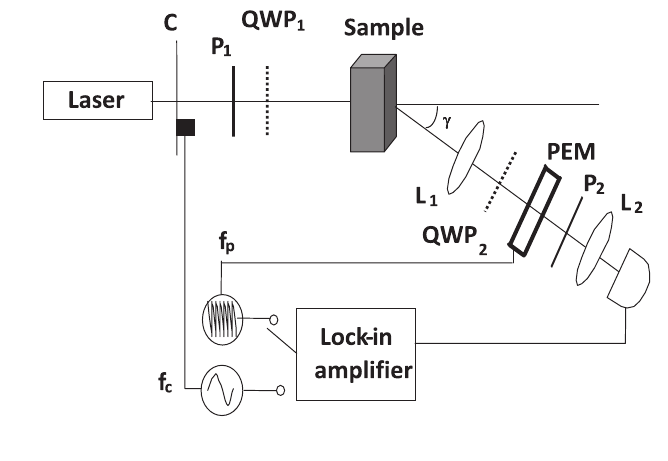
\includegraphics[width = 0.6\textwidth]{Chapter4/Figures/PMSDpolarimetry.png}	
%	\caption{ A schematic of the experimental polarimetry system with a polarization modulation and synchronous detector \cite{guo2006angular}}
%	\label{fig:PMSDpolarimetry}
%	\end{figure}

	
\subsection{Mueller polarimeter}
As explained earlier, Stokes vectors are not enough for measuring medium properties, so additional measurements and analysis is required.
The Mueller matrix provides these additional measurements at the cost of a more complicated setup.
This matrix and its parameters were explained in Sect.\,\ref{subsec:MuellerMeasurement}.
Sixteen elements of the Mueller matrix are measured via \acf{dc} sequential static measurements or \acf{ac} modulation based measurements \cite{ghosh2011tissue}.
In the latter approach, the four states of polarization (linear polarization at $0^{\circ}$, $45^{\circ}$, $90^{\circ}$ and rigth/left circular polaization $L$ and $R$) are applied individually as the input state, and the Stokes vector corresponding to each input is measured as an output.
The 16 elements of the Mueller matrix are then constructed using the measured Stokes vectors (see Eq. \ref{Eq:MuellerPolarimetry}) \cite{ghosh2009mueller}. 
	
	\begin{equation}\label{Eq:MuellerPolarimetry}
	\small
	M = 
	\begin{bmatrix}
	\frac{1}{2}(I_{H}+I_{V}) &  \frac{1}{2}(I_{H}-I_{V}) &  I_{P}-M(1,1) &  I_{R}-M(1,1)\\
    \frac{1}{2}(Q_{H}+Q_{V}) &  \frac{1}{2}(Q_{H}-Q_{V}) &  Q_{P}-M(2,1) &  Q_{R}-M(2,1)\\
	\frac{1}{2}(U_{H}+U_{V}) &  \frac{1}{2}(U_{H}-U_{V}) &  U_{P}-M(3,1) &  U_{R}-M(3,1)\\
	\frac{1}{2}(V_{H}+V_{V}) &  \frac{1}{2}(V_{H}-V_{V}) &  V_{P}-M(4,1) &  V_{R}-M(4,1)\\		
	\end{bmatrix}~,
	\end{equation}\\
	
\noindent where the four input states are denoted with $H$ for $0^{\circ}$, $V$ for $ 90^{\circ}$, $P$ for $45^{\circ}$, and $R$ for right circular polarized.
The Mueller matrix elements are represented by $M(i,j)$ with respect to their row and column.
This approach has been used by \cite{ghosh2009mueller,ghosh2008mueller}.
%The modulation/synchronous detection approach explained for Stokes polarimeter, can be used for Mueller polarimeter as well \cite{ghosh2009mueller,ghosh2009mueller}.

A dual rotating retarder approach is another way to generate the modulation-based Mueller matrix polarimeters \cite{ghosh2011tissue,goldstein1992mueller,azzam1978photopolarimetric,smith2002optimization}.
In this approach, the incident polarization states are generated by the \ac{psg} unit which contains a linear polarizer and a rotating linear retarder with retardance and angular speed of $\sigma_{1}$ and $\omega_{1}$, respectively.
The backscattered light from the sample are then analyzed by a \ac{psa} unit.
This unit contains a rotating linear retarder (retardance of $\sigma_{2}$ and angular speed of $\omega_{2}$) and a fixed linear polarizer in sequence.
In this set-up the axis of the polarizer and analyzer are kept parallel and the retardation of the two retarders is chosen to be the same $\sigma_{1} = \sigma_{2}= \pi/2$, while their angular frequencies differ from each other by five times ($\omega_{1} = \omega$, $\omega_{2} = 5\omega$ ).
The rotation of the retarders at different rates results in a modulation of a detected signal and encodes all the sixteen Mueller matrix elements into the amplitude and phases of 12 frequencies in the detected intensity signal.
The detected signal is Fourier analyzed and the Mueller matrix elements are constructed from the Fourier coefficients \cite{ghosh2011tissue,goldstein1992mueller,azzam1978photopolarimetric,smith2002optimization}. 

Dubreuil~et al.\,\cite{dubreuil2007snapshot} introduced another modulation-based Mueller matrix polarimeter, known as the Snapshot Mueller matrix.
The Snapshot system contains two linear birefringence retarders (wave plates) and a linear polarizer in the \ac{psg} unit and two birefringence retarders and a fixed linear polarizer (perpendicular to the one in the \ac{psg} unit) at the \ac{psa} unit (see Fig. \ref{fig:snaphotMueller}).
This technique measures the 16 elements of the Mueller matrix simultaneously by using wavelength polarization coding and decoding.
The resultant spectral signal is stored by the spectrometer and is Fourier analyzed in order to achieve the 16 elements of the Mueller matrix. 
	\begin{figure}
	\centering 
	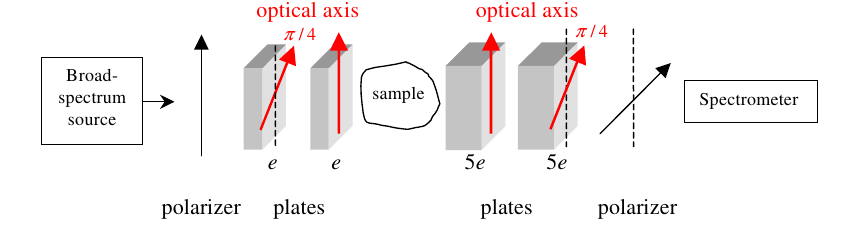
\includegraphics[width = 0.7\textwidth]{Chapter4/Figures/snapshotMueller.png}	
	\caption{ Snapshot Mueller polarimeter for the configuration, \cite{dubreuil2007snapshot}. }
	\label{fig:snaphotMueller}
	\end{figure}
\noindent In this system the \ac{psg} unit contains a linear polarizer at \ang{0} and two wave plates with their axis rotated at \ang{45} and \ang{0}, respectively.
The \ac{psa} unit contains two wave plates with their axis at \ang{0} and \ang{45}, respectively, and a linear polarizer at \ang{90}. 
One crucial parameter in this system is the choice of thickness of the birefringence plates.
The author proposed to having the birefringence in the \ac{psa} unit five times thicker than those in the \ac{psg}.

It should be noted that the Mueller polarimeters mentioned so far are suited for point polarimetry and are not applicable for large area imaging.
In this regard, several approaches are proposed and explained in the following.

Antonelli~\cite{antonelli2011biomedical} proposed three Mueller image polarimeters in her phd thesis; full Mueller imaging using focused illumination, Fourier space image polarimetry, and real space full Mueller imaging.
The latter system was proposed for thick tissue imaging while the two former, ones were designed for thinner tissue.
The first proposed instrument is shown in Fig.~\ref{fig:FIMueller}.
This system was implemented according to the system described by \cite{hielscher1997diffuse}.
Hielscher~et al.\,\cite{hielscher1997diffuse} developed the Mueller imaging system for analyzing the intensity patterns of backscattered light from the turbid media.
\begin{figure}[H]
\begin{center}
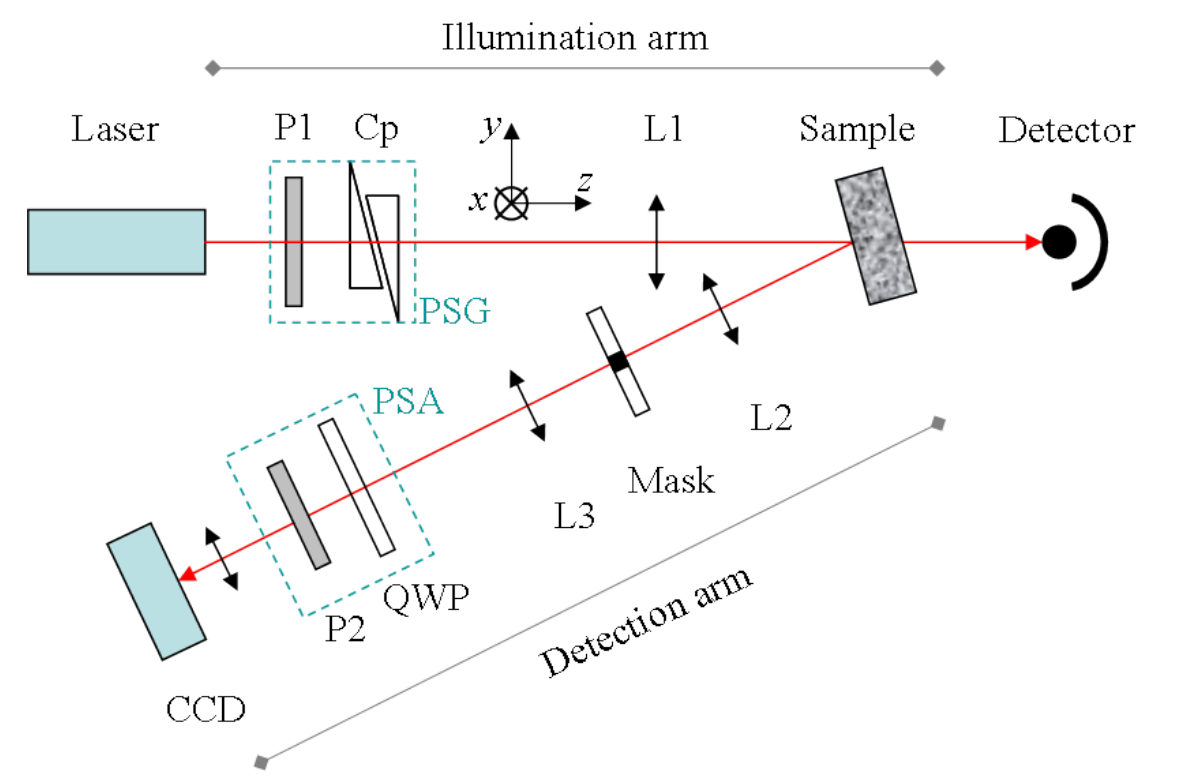
\includegraphics[width = 0.7\textwidth] {Chapter4/Figures/FIMueller.png}
\end{center}
\caption[Full Mueller polarimetry using focused illumination~\cite{antonelli2011biomedical}]{Full Mueller polarimetry system with focused illumination. The image is taken from \cite{antonelli2011biomedical}.}
\label{fig:FIMueller}
\end{figure}
\noindent The \ac{psg} unit of this system is composed of a linear polarizer ($P_{1}$) and a Babinet-Soleil-Bravais compensator (CP)~\cite{antonelli2011biomedical}, while the \ac{psa} unit is composed of a quarter wave plate (QWP) and a linear polarizer ($P_{2}$).
The compensator retardance is set to either \ang{180}, or \ang{90}.
The former is used to generate the linearly polarized states, and the later to generate circular polarized states.
In the \ac{psa} unit the QWP is set parallel to $P_{2}$ to measure the linear polarized state and it is rotated by \ang{45} to measure circular polarized states.
Using this setup, 36 raw images, corresponding to all the combinations of the polarization states possible in the \ac{psg} and \ac{psa} units, are acquired to complete the Mueller matrix. 
The final Mueller matrix, as a combination of the acquired 36 images, is shown in Fig.~\ref{fig:FIMuellermat}.
Here $O$ refers to an unpolarized state which is generated by the average of the two orthogonal state (i.e. H and V or P and M or L and R).
For each pair, for instance $HV$, the first element represents the polarization state of the \ac{psg} unit, while the polarization state of the \ac{psa} unit is represented by the second element.
\begin{figure}
\begin{center}
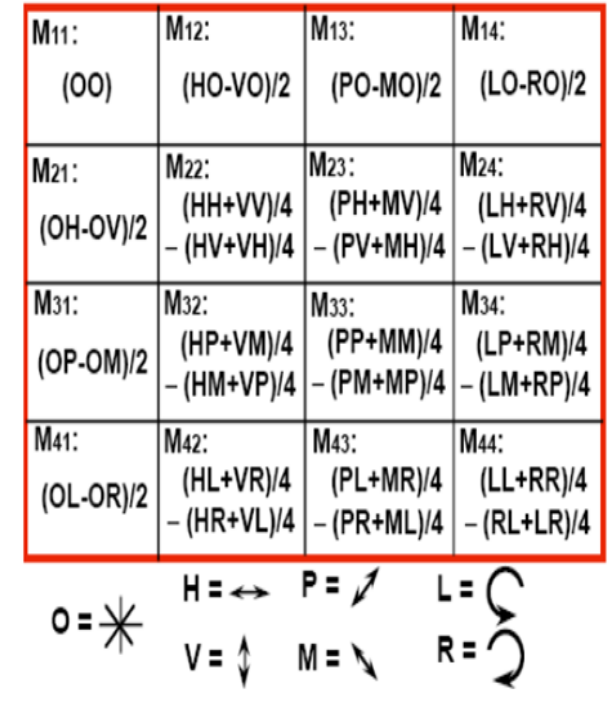
\includegraphics[width = 0.6\textwidth ]{Chapter4/Figures/FIMuellermat.png}
\end{center}
\caption[Mueller matrix obtained by full Mueller imaging with focused illumination system~\cite{antonelli2011biomedical}]{Mueller matrix as combination of 36 raw images acquired by full Mueller imaging with focused illumination setup~\cite{antonelli2011biomedical}.}
\label{fig:FIMuellermat}
\end{figure}

The second system, Fourier space image polarimetry, is shown in Fig.~\ref{fig:FSMueller}.
In this system, the \ac{psg} unit consists of a half wave plate (HWP), followed by a linear polarizer and QWP and the \ac{psa} unit contains one QWP followed by a linear polarizer.
Table~\ref{tab:AntonelliTable} illustrates the existence and rotation of each of the optic elements in the \ac{psg} and \ac{psa} units for creating different polarization states.
It should be noted that the polarization states generated in the \ac{psg} unit are independent from those generated in the \ac{psa} unit.

\begin{table}
\caption[Polarized state generator and \ac{psa} units setting proposed by \cite{antonelli2011biomedical}]{Setting for the \ac{psg} and \ac{psa} units for generating 6 polarization states in each unit~\cite{antonelli2011biomedical}.}
\begin{center}
\scriptsize{
\resizebox{0.7\textwidth}{!}{
\begin{tabular}{c ccc c	cc}
\toprule 
 & \multicolumn{3}{c}{\ac{psg}} &  & \multicolumn{2}{c}{\ac{psa}}\\
 \cmidrule{2-4} \cmidrule{6-7}
Polarization states & HWP & P & QWP & & QWP & P \\
\midrule
H & \ang{0} & \ang{0} & removed & & removed & \ang{0}\\
V & \ang{45} & \ang{90} & removed & & removed & \ang{90}\\
P & \ang{45} & \ang{45} & removed & & removed & \ang{45}\\
M & \ang{45} & \ang{315} & removed & & removed & \ang{135}\\
R & \ang{45} & \ang{90} & \ang{45} & & \ang{45} & \ang{0}\\
L & \ang{45} & \ang{90} & \ang{-45} & & \ang{-45} & \ang{90}\\
\bottomrule

\end{tabular}}}
\end{center}
\label{tab:AntonelliTable}
\end{table}

\begin{figure}
\begin{center}
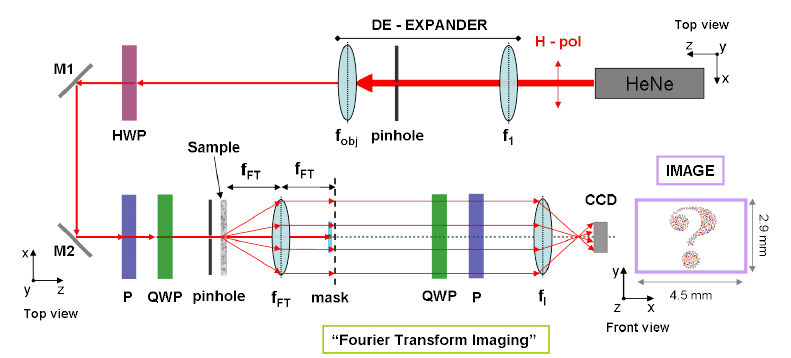
\includegraphics[width = 0.9\textwidth]{Chapter4/Figures/FourierTransformImaging.png}
\end{center}
\caption[Fourier space Mueller polarimetry~\cite{antonelli2011biomedical}]{ Fourier space Mueller polarimetry system proposed by \cite{antonelli2011biomedical}.}
\label{fig:FSMueller}
\end{figure}
\noindent Using the 36 raw images with different polarization states, the author also proposed using a so called polarimetric matrix ($6 \times 4$), whose columns are the components of the normalized Stokes vector and the lines are the input polarization states (see Fig.~\ref{fig:PM}).
Similar to the Mueller matrix (see Fig.~\ref{fig:FIMuellermat}), the polarization state of the \ac{psg} unit is represented by the first element while the second element shows the polarization state of the \ac{psa} unit.
	\begin{figure} [h]
	\centering 
	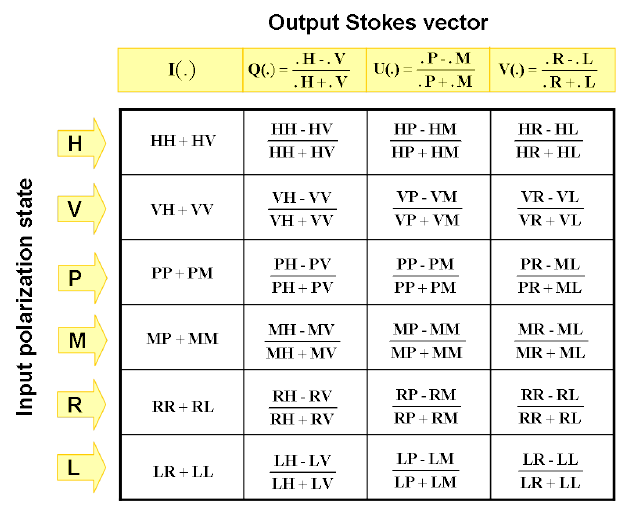
\includegraphics[width = 0.8\textwidth]{Chapter4/Figures/PolarimetricMatrix.png}	
	\caption[Polarimetric matrix]{Polarimetric matrix defined with Fourier space imaging~\cite{antonelli2011biomedical}. }
	\label{fig:PM}
	\end{figure}
	
The third system, real space full Mueller imaging, similar to \cite{de2004general} uses two \ac{lc} to eliminate the need of manual rotation of the optical parts in the \ac{psg} and \ac{psa} units (see Fig.~\ref{fig:RSMueller}).
This system was used for imaging ex-vivo cone biopsies.
	\begin{figure}[h]
	\centering 
	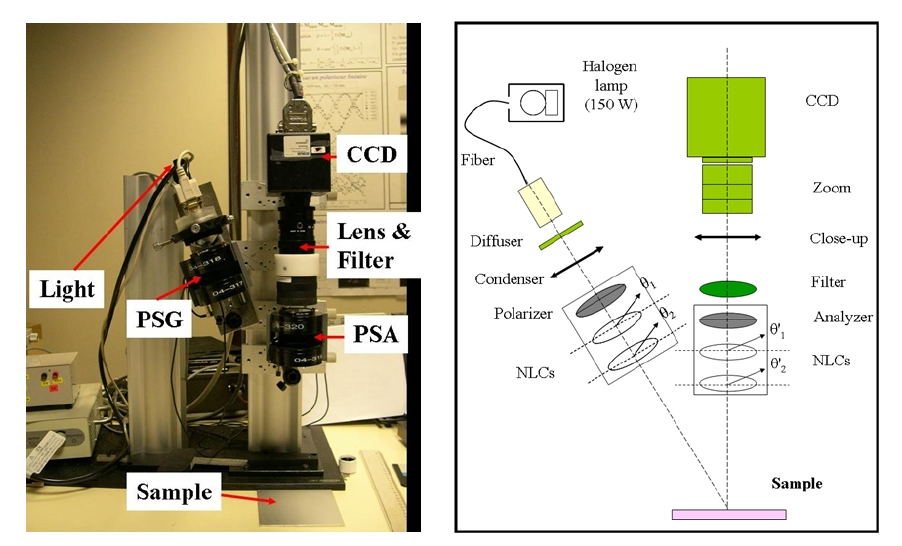
\includegraphics[width = 0.9\textwidth]{Chapter4/Figures/RealMuellerImagingSystem.png}	
	\caption[Real spape Mueller imaging proposed by \cite{antonelli2011biomedical}]{ The real space Mueller imaging system proposed by \cite{antonelli2011biomedical}. }
	\label{fig:RSMueller}
	\end{figure}

\noindent In this system, the \ac{psg} unit consists of a linear polarizer and two \ac{lc} elements and the \ac{psa} unit contains the same elements in reverse order (i.e. two \ac{lc} and then a linear polarizer).
Using different rotation angles for the two \ac{lc} allows to obtain the four polarization states for the \ac{psg} and \ac{psa} units (common choice of angles, $\theta_{1} = \ang{45}$, and $\theta_{2} = \ang{0}$).
Consider the four incident polarization states of the \ac{psg} unit as $4 \times 4$ matrix $W$ (polarization states as columns) and the four basic states of the \ac{psa} unit as $4 \times 4$ matrix $A$ (polarization states as rows).
Then the 16 raw data are the elements of a $4 \times 4$ real matrix $B$ (measurement matrix) such as~\cite{de2004general, antonelli2011biomedical}:
	\begin{equation}
	\label{eq:LCMuellerEq}
	B = AMW~,
	\end{equation}
\noindent where $M$ is the Mueller matrix of the sample.
Having the initial knowledge of the $A$ and $W$ matrices and measuring the $B$ matrix, the Mueller matrix $M$ is calculated.
The two matrices of $A$ and $W$ are known through the calibration procedure~\cite{compain1999general}.
%This matrix is obtained by measuring the $B$ matrix and  which can be calculated by measuring the $B$ matrix and having the initial knowledge of $A$ and $W$.
%The two matrices of $A$ and $W$ are known if the system is calibrated~\cite{compain1999general}.

Besides the aforementioned systems, Mueller polarimetry was used in several other studies to capture images of human and animal tissues~\cite{twietmeyer2008mueller,li2009mueller}.

Li~et al.\,\cite{li2009mueller} proposed another ex-vivo instrument to characterize muscle depolarization properties.
Comparing relax and stretch muscles and polystyrene solution, the authors concluded that the polarization properties of a muscle are clearly different from the polystyrene solution.
However, despite clear changes in raw polarization references, muscle stretching shows minimal changes in terms of its polarization properties. 

Twietmeyer~et al.\,\cite{twietmeyer2008mueller} proposed a Mueller polarimetry system for in-vivo imaging of the retina and tested their proposed method on 15 normal subjects.
The authors proposed adjusting the available scanning laser polarimeter GDx by using two \ac{lc} in the \ac{psg} and \ac{psa} units in order to change the polarization states.
Although no subjects with retinal diseases were evaluated, the authors concluded that the proposed system is well suited for monitoring the thickness of the nerve fiber and Henle layers and can be used as an indicator of the presence and progression of glaucoma~\cite{twietmeyer2008mueller}.




% Such a system will have lower sensitivity so alternative methods have been considered for instance using a liquid crystal variable retarders ($LC$) instead of manually rotating the optical parts of the PSG and PSA \cite{de2004general} (see Fig \ref{fig:LCMueller}).  The PSG unit of this system consists of a linear polarizer ($P_{1}$) and two liquid crystal variable retarders ($LC_{1}$, $LC_{2}$) with two retardance value of $\sigma_{1}$ and $\sigma{2}$ respectively. The PSA unit have a similar structure to PSG unit ($LC_{3}$, $LC_{4}$ and $P_{2}$) with the reverse order and the detection device at the end, in this case a CCD, for image acquisition. The structure of the LC polarimeter can be seen in Fig \ref{fig:LCMueller}.
%	\begin{figure} 
%	\centering 
%	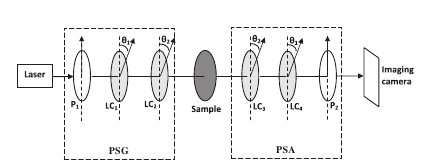
\includegraphics[width = 0.8\textwidth]{Chapter4/Figures/LCMueller.png}	
%	\caption{$LC$ Mueller matrix polarimeter \cite{ghosh2011tissue} }
%	\label{fig:LCMueller}
%	\end{figure}

%Usually the birefringence axis of the two retarders are kept at angles $\theta_{1}$ and $\theta_{2}$ respectively with reference to the axis of the polarizer $P_{1}$. (Generally the angles are chosen as: $\theta_{1} = 45 ^{\circ}$ and $\theta_{2} = 0 ^{\circ}$). Considering the optics elements order in the PSG unit, once can conclude how the incident polarizer states can be related to $\sigma_{1}$ and $\sigma_{2}$. This relation is illustrated in Eq.\ref{Eq:LCMuellerEq}.
%
%	\begin{equation}\label{Eq:LCMuellerEq}
%	\small
%	\begin{pmatrix} 
%	I_{f}\\
%	Q_{f}\\
%	U_{f}\\	
%	V_{f}\\
%    \end{pmatrix} = 		
%	\begin{pmatrix}
%	1 & 0 & 0 & 0 \\
%	0 & 1 & 0 & 0 \\
%	0 & 0 & \cos \sigma_{2} &  \sin \sigma_{2}\\
%	0 & 0 & -\sin \sigma_{2} &  \cos \sigma_{2}\\
%	\end{pmatrix}
%	\begin{pmatrix}
%	1 & 0 & 0 & 0 \\
%	0 & \cos \sigma_{1} & 0 & -\sin \sigma_{1} \\
%	0 & 0 & 1 & 0 \\
%	0 & \sin \sigma_{1} & 0 & \cos \sigma_{1} \\
%	\end{pmatrix} 
%	\begin{pmatrix}
%	1\\
%	1\\
%	0\\
%	0\\
%	\end{pmatrix} = 
%	\begin{pmatrix}
%	1 \\
%	\cos\sigma_{1}\\	
%	\sin \sigma_{2} \sin \sigma_{1}\\	
%	\cos \sigma_{2} \sin \sigma_{1}\\
%	\end{pmatrix}	
%	\end{equation} 

%%%The calibration of a system like the imaging polarimeter we are describing is a very
%%%difficult task by the usual approach involving a detailed model of the instrument, as this
%%%system is a "stack" of many elements, each of which may introduce serious artefacts which
%%%may be difficult to understand and model properly.
%%%A very different approach has been followed at LPICM [70] to develop the eigenvalue
%%%calibration method (ECM), which has been successfully used on many different Mueller
%%%polarimeters. Without getting into details, which would be outside the scope of this
%%%manuscript, this method can accurately retrieve the matrices W and A from four mea-
%%%surements on calibration samples by linear algebra techniques, without any modelling of
%%%the instruments. Moreover, the calibration samples are not very specific (typically one
%%%can use linear polarizers, retardation plates other than half wave) and do not need to be
%%%accurately known, as they are characterized during the calibration procedure itself. Of
%%%course, our imaging polarimeter was calibrated at each wavelength by using ECM, and
%%%provided polarimetric images with a typical maximum error of the order of 0.02 to 0.03
%%%on the normalized elements Mij ∗
%%% = Mij /M11, i, j = 1..4 i · j = 1.

%	\begin{figure}
%	\begin{center}
%	\subfloat[]{
%	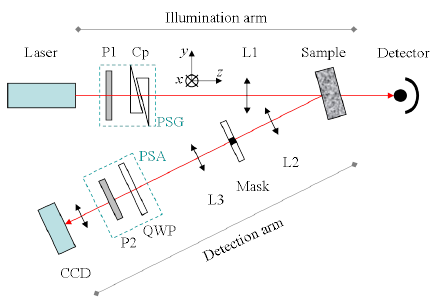
\includegraphics[width = 0.7\textwidth]{Chapter4/Figures/illuminationMueller.png}
%	\label{fig:focusedMueller}
%	}\  \\
%	\subfloat[]{%[width=0.3\textwidth]
%    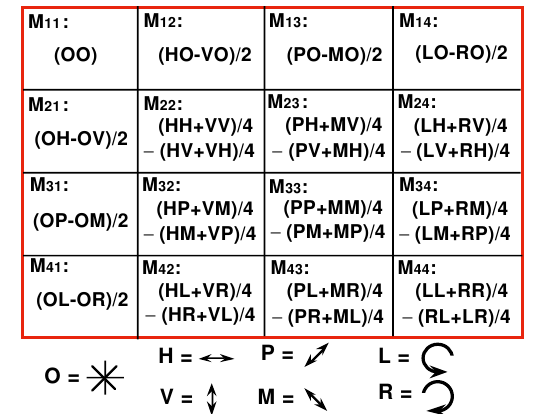
\includegraphics[width = 0.7\textwidth]{Chapter4/Figures/illuminationMueller_table.png}
%    \label{fig:illuminationMuellerTable}
%	}
%	\caption{(a)Full Mueller imaging system (b) Combination of the raw images for calculating the Mueller matrix elements   \cite{antonelli2011biomedical,hielscher1997diffuse}} 	
%	\end{center}
%	\end{figure}










